\documentclass{beamer}
%
% Choose how your presentation looks.
%
% For more themes, color themes and font themes, see:
% http://deic.uab.es/~iblanes/beamer_gallery/index_by_theme.html
%
\mode<presentation>
{
  \usetheme{Boadilla}      % or try Darmstadt, Madrid, Warsaw, ...
  \usecolortheme{default} % or try albatross, beaver, crane, ...
  \usefonttheme{default}  % or try serif, structurebold, ...
  \setbeamertemplate{navigation symbols}
} 

\usepackage[english]{babel}
\usepackage[utf8x]{inputenc}
\usepackage{pdfpages}
\usepackage{float}

\newenvironment<>{varblock}[2][.9\textwidth]{%
  \setlength{\textwidth}{#1}
  \begin{actionenv}#3%
    \def\insertblocktitle{#2}%
    \par%
    \usebeamertemplate{block begin}}
  {\par%
    \usebeamertemplate{block end}%
  \end{actionenv}}

\title[Neuroanatomy workshop 3]{The Sensory-motor System}
\author{JJ Torre}
\institute{Parietal Team - INRIA Saclay}
\date{2018}

\begin{document}

\begin{frame}
  \titlepage
\end{frame}

% Uncomment these lines for an automatically generated outline.
%\begin{frame}{Outline}
%  \tableofcontents
%\end{frame}

\section{Introduction}

\begin{frame}{Introduction}
 \begin{columns}[T]
  \begin{column}{.4\textwidth}
    \begin{itemize}
      \item The sensory-motor system constitutes our main means of receiving input (sensory
      stimuli) and producing output (movement) in relation to the environment
      \item It follows a hierarchical organization common to both motor and sensory systems
    \end{itemize}

    \vspace{-.3cm}
    \begin{varblock}[5cm]{\scriptsize Peripheral Nervous System (PNS)}
     \scriptsize Although we are going to focus on the central nervous system, a lot is going on before reaching the brain! Motor reflexes happen at this level
    \end{varblock}
  \end{column}
  \begin{column}{.6\textwidth}
   \begin{figure}[H]
   \vspace*{-1.25cm}
    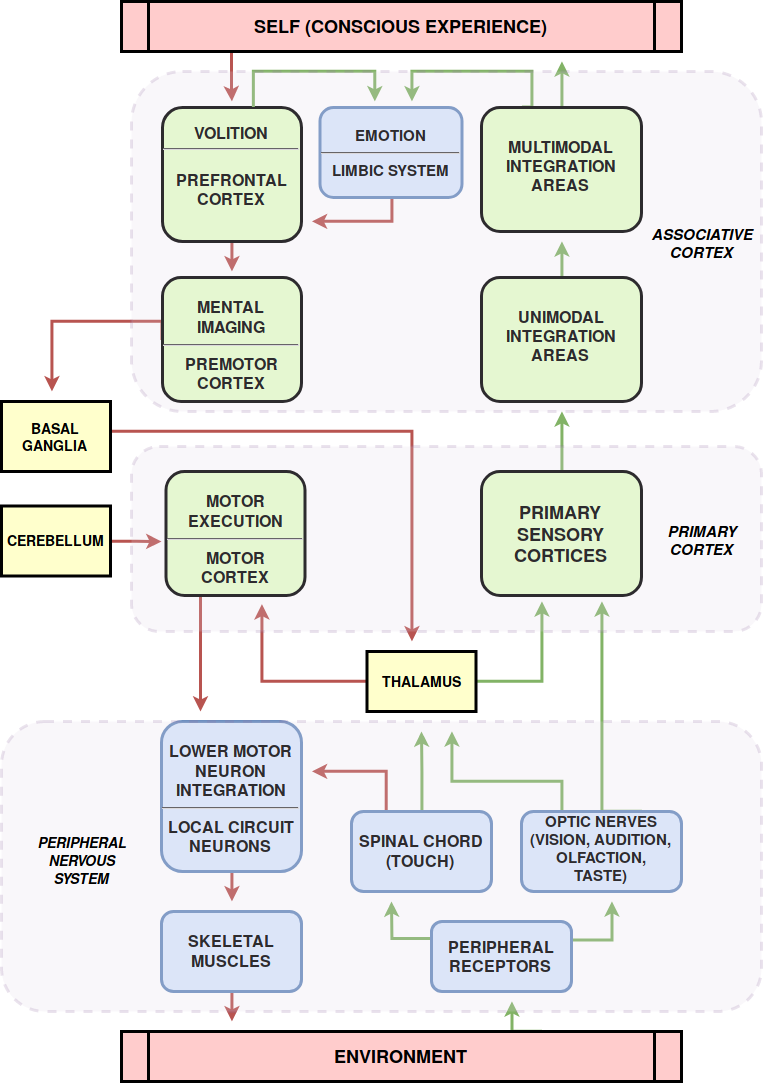
\includegraphics[width=.85\textwidth]{figures/brain_and_env.png}
   \end{figure}
  \end{column}
 \end{columns}
\end{frame}

\begin{frame}{Primary Areas}
 \begin{columns}[T]
  \begin{column}{.4\textwidth}
    \begin{itemize}
      \item \small Primary areas receive input directly from the thalamus
      \item \small Sensory areas receive high-dimensional data for each modality (vision, audition, etc.)
      \item \small The motor cortex conveys the already planned movement and sends it to the muscles
      \item \small Primary cortices have the better and most differentiated 6-layer laminar structure
    \end{itemize}
  \end{column}
  \begin{column}{.6\textwidth}
   \begin{figure}[H]
    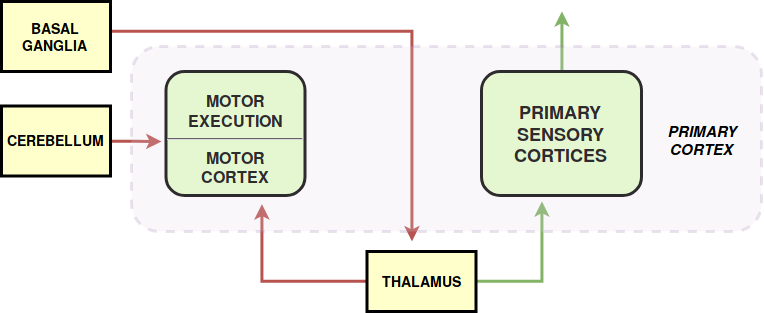
\includegraphics[width=1\textwidth, height=3.5cm]{figures/primary_structures.png}
   \end{figure}
   \vskip
   \begin{varblock}[7cm]{\scriptsize Olfaction is a special boy}
    \scriptsize Olfaction is the only sense that does not do thalamic relay in its
    path to the cortex. Signals from the nose go directly to the piriform cortex via the
    olfactory tract.
   \end{varblock}
  \end{column}
 \end{columns}
\end{frame}

\begin{frame}{Associative areas}

 \begin{columns}[T]
  \begin{column}{.4\textwidth}
    \begin{itemize}
      \item \small Can receive input from a diverse range of cortical areas
      \item \small As we go up on the hierarchy, it becomes ingreasingly difficult to pin down specific processes to brain regions
      \item \small There are two different sub-categories of associative areas: secondary (premotor cortex/unimodal integration areas) and tertiary (prefrontal cortex/multimodal integration)
    \end{itemize}
  \end{column}
  \begin{column}{.6\textwidth}
   \begin{figure}[H]
    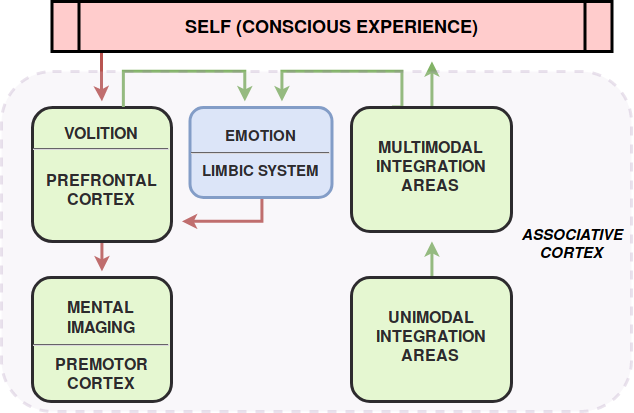
\includegraphics[width=.8\textwidth, height=3.5cm]{figures/associative_cortex.png}
    \end{figure}
   \vskip
   \begin{varblock}[7cm]{\scriptsize Neuroscientists do not agree on anyting - Part I}
    \scriptsize Although sometimes the term "associative" is used to designate all the cortex that is not a primary area, here we are referring only to sensory and motor association cortices.
   \end{varblock}
  \end{column}
 \end{columns}
\end{frame}

\begin{frame}{Secondary areas}

    \begin{itemize}
      \item They receive input mostly from their respective primary (sensory) or tertiary (motor) areas
      \item Secondary sensory areas show asymmetry patterns within each modality (more on that later)
      \item Secondary or premotor areas are mostly involved in the integration of all elements needed to perform movements
    \end{itemize}
    
\end{frame}

\begin{frame}{Tertiary areas}

    \begin{itemize}
      \item They constitute the link between higher cognition and their corresponding sensorimotor systems
      \item Information integrated from cognition that results in movement is feeded to secondary motor areas from tertiary motor areas, whereas tertiary sensory areas feed sensory representations to a variety of cortical areas
      \item The thalamus plays a crucial role in the widespread distribution both to and from these areas
      \item Processing in these areas does not involve perception or motor activities. Rather, they take charge of issue movements or integrate sensory representations across different sensory modalities.
    \end{itemize}

\end{frame}

\end{document}
